\documentclass[10pt]{beamer}
\usepackage[latin1]{inputenc}
\usepackage{amsmath}
\usepackage[T1]{fontenc}
\usepackage{ stmaryrd }
\usepackage{amsfonts}
\usepackage{amssymb}
\usepackage{upquote}
\usepackage{listings}
\usepackage{ulem}
\usetheme{Antibes}
\lstset{language=Haskell}
\lstset{breaklines=true}
\lstset{frame=single}
\lstset{frameround=tttt}

\definecolor{olivegreen}{HTML}{8DC73E}

\newcommand\doubleplus{+\kern-1.3ex+\kern0.8ex}
\newcommand\mdoubleplus{\ensuremath{\mathbin{+\mkern-10mu+}}}

\newcommand\monadbind{\gg\!\!=}

\author{
	Ralf Hinze\\
	\ \\
	\ \\
	\
	Presented by Beerend Lauwers\\
	\
	Utrecht University, The Netherlands
}
\date{\today}
\title{Typed Quotation / Antiquotation in Haskell
	    \newline ~Or: Compile-time parsing}

\begin{document}

\frame{\maketitle}

\begin{frame}{Outline}
\tableofcontents
\end{frame}

\section{Quotation/Anti-quotation: short introduction}
\subsection{Quotation}
\begin{frame}[fragile]{Quotation: short introduction}

\begin{itemize}
\item \textbf{Quotation} allows you to integrate a guest language into a host language:

\begin{lstlisting}[mathescape=true]
	Main$\rangle$ $\ll$ $\texttt{fork fork leaf leaf leaf}$ $\gg$
	Fork (Fork Leaf Leaf) Leaf
	Main$\rangle$ size $\ll$ $\texttt{fork fork leaf leaf leaf}$ $\gg$ + 1 
	4
\end{lstlisting}

\item A quotation is surrounded by guillemets: $\ll$ $\gg$

\item A quotation evaluates to an abstract syntax.

\item Great for EDSLs!

\end{itemize}

\end{frame}

\subsection{Anti-quotation}
\begin{frame}[fragile]{Anti-quotation: short introduction}

\begin{itemize}
\item With \textbf{anti-quotation}, we can use the host language in the guest language:

\begin{lstlisting}[mathescape=true]
	Main$\rangle$ $\ll$ $\texttt{fork}$ `(full 2) $\texttt{leaf}$ $\gg$
	Fork (Fork (Fork Leaf Leaf) (Fork Leaf Leaf)) Leaf
\end{lstlisting}

\item An anti-quotation begins with a backtick and usually evaluates to an abstract syntax.

\end{itemize}

\end{frame}

\subsection{Implementation in GHC}
\begin{frame}[fragile]{Quotation/Anti-quotation: implementation in GHC}

\begin{itemize}
\item The language needs to be extended to support quotation/anti-quotation.
\item GHC provides the \textbf{Quasiquotation} extension.
\item This extension uses Template Haskell, which suffers from typing issues.
\end{itemize}

\begin{center}
\textbf{Could we implement this functionality in plain Haskell?}
\end{center}

\end{frame}

\begin{frame}[fragile]{Quotation/Anti-quotation: implementation in GHC}

\begin{itemize}
\item The language needs to be extended to support quotation/anti-quotation.
\item GHC provides the \textbf{Quasiquotation} extension.
\item This extension uses Template Haskell, which suffers from typing issues.
\end{itemize}

\begin{center}
\textbf{Could we implement this functionality in plain Haskell?}

Indeed, we can. That's what this paper's about.
\end{center}

\end{frame}

\begin{frame}[fragile]{Quotation/Anti-quotation: implementation in GHC}

\begin{itemize}
\item The language needs to be extended to support quotation/anti-quotation.
\item GHC provides the \textbf{Quasiquotation} extension.
\item This extension uses Template Haskell, which suffers from typing issues.
\end{itemize}

\begin{center}
\textbf{Could we implement this functionality in plain Haskell?}

Indeed, we can. That's what this paper's about.
\end{center}
\begin{center}
\textbf{Assumption:} arbitrary terminal symbols in \texttt{typewriter} font are Haskell identifiers (!)
\end{center}

\end{frame}

\section{A simple example}
\subsection{DSL for natural numbers}
\begin{frame}[fragile]{Example: DSL for natural numbers}

\begin{itemize}
\item Simple example: a DSL for natural numbers:

\begin{lstlisting}[mathescape=true]
	Main$\rangle$ ($\ll$ | | | $\gg$,$\ll$ | | | | | $\gg$ + 7)
	(3,12)
\end{lstlisting}

\item Let's define some aliases to help us decipher this:
\begin{itemize}
	\item $\ll$ = quote
	\item $\gg$ = endquote
	\item $|$ = tick
\end{itemize}

\item Then,

\begin{lstlisting}[mathescape=true]
	$\ll$ | | | $\gg$
\end{lstlisting}

becomes

\begin{lstlisting}[mathescape=true]
	(((quote tick) tick) tick) endquote
\end{lstlisting}

\end{itemize}

\end{frame}

\begin{frame}[fragile]{Example: DSL for natural numbers}

\begin{itemize}

\begin{lstlisting}[mathescape=true]
	(((quote tick) tick) tick) endquote
\end{lstlisting}

\item How can we evaluate this?

\begin{lstlisting}[mathescape=true]
	quote f = f 0
	tick n f = f (succ n)
	endquote n = n
\end{lstlisting}

\item Stepwise evaluation:

\begin{lstlisting}[mathescape=true]
	quote tick tick tick endquote
	= tick 0 tick tick endquote
	= tick 1 tick endquote
	= tick 2 endquote
	= endquote 3
	= 3
\end{lstlisting}

\item Evaluation is driven by terminal symbols = \textbf{active terminals}.
% Write down terminals drive evaluation = active terminals on board

\end{itemize}

\end{frame}

\subsection{The CPS Monad}

\begin{frame}[fragile]{The CPS Monad}

\begin{itemize}

\item This looks a lot like \textbf{continuation-passing style (CPS)}...
\item Indeed, we can make it an instance of the CPS monad:

\begin{lstlisting}[mathescape=true]
	type CPS $\alpha$ = $\forall$ans.($\alpha \rightarrow $ans)$\rightarrow$ans
	instance Monad CPS where
	  return a = $\lambda \kappa \rightarrow \kappa$ a
	  m $\monadbind$ k     = $\lambda \kappa \rightarrow$m ($\lambda$a$\rightarrow$k a $\kappa$)
\end{lstlisting}

\item Then, 
\begin{lstlisting}[mathescape=true, escapechar=!]
	quote = return 0
	= $\lambda \kappa \rightarrow \kappa$ 0
	!\textcolor{olivegreen}{- - Original: quote f = f 0)}!
	tick = lift succ = $\lambda$a$\rightarrow$return (succ a)
	= $\lambda$a$\rightarrow\lambda \kappa \rightarrow \kappa$ (succ a)
	!\textcolor{olivegreen}{- - tick n f = f (succ n))}!
\end{lstlisting}

\end{itemize}

\end{frame}

\begin{frame}[fragile]{The CPS Monad}

\begin{itemize}

\item This looks a lot like \textbf{continuation-passing style (CPS)}...
\item Indeed, we can make it an instance of the CPS monad:

\begin{lstlisting}[mathescape=true, escapechar=!]
	type CPS $\alpha$ = $\forall$ans.($\alpha \rightarrow $ans)$\rightarrow$ans
	instance Monad CPS where
	  return a = $\lambda \kappa \rightarrow \kappa$ a
	  m $\monadbind$ k     = !\color{red}{m k}!
\end{lstlisting}

\item Then, 
\begin{lstlisting}[mathescape=true, escapechar=!]
	quote = return 0
	= $\lambda \kappa \rightarrow \kappa$ 0
	!\textcolor{olivegreen}{- - Original: quote f = f 0)}!
	tick = lift succ = $\lambda$a$\rightarrow$return (succ a)
	= $\lambda$a$\rightarrow\lambda \kappa \rightarrow \kappa$ (succ a)
	!\textcolor{olivegreen}{- - tick n f = f (succ n))}!
\end{lstlisting}

\end{itemize}

\end{frame}

\begin{frame}[fragile]{The CPS Monad}

\begin{itemize}

\item So, the quotation \begin{lstlisting}[mathescape=true]
	$\ll$ | | | $\gg$
\end{lstlisting}
can be written as a monadic computation:
\begin{lstlisting}[mathescape=true, escapechar=!]
	run (quote $\monadbind$ tick $\monadbind$ tick $\monadbind$ tick)
\end{lstlisting}

\item (run encapsulates a CPS computation:)
\begin{lstlisting}[mathescape=true, escapechar=!]
	run :: CPS $\alpha \rightarrow \alpha$
	run m = m id
\end{lstlisting}

\end{itemize}

\end{frame}

\begin{frame}[fragile]{The CPS Monad}

\begin{itemize}

\item Generalizing:
\begin{lstlisting}[mathescape=true]
	(((quote act$_1$) ...) act$_n$) endquote
	=
	run (quote $\monadbind$ act$_1$ $\monadbind$ ... $\monadbind$ act$_n$) 
\end{lstlisting}
where
\begin{lstlisting}[mathescape=true]
	quote :: CPS$\tau_1$
	act$_i$   :: $\tau_i \rightarrow$ CPS$\tau_{i+1}$
	endquote = id
\end{lstlisting}
% quote initializes the state
% act_i is a transition to another state, each active terminal transforms the state

\item In this example, there was only a single state type.
\item Choosing your state types carefully is very important, as we shall see later on.
% In this case, there is a single state type, but we can have more than one.

\item Note: endquote can be any function, not just the identity:
\begin{lstlisting}[mathescape=true]
	postProcess (run m)
\end{lstlisting}

\end{itemize}

\end{frame}

\begin{frame}[fragile]{Next up: parsers in CPS monad}

\begin{itemize}

\item So, evaluation of a quotation is driven by the terminals.
\item For a specific guest language, we need a specific parser for the concrete syntax.
\item We'll look at three types of parsers, ordered by complexity:
\begin{itemize}
\item Simple postfix and prefix parsers
\item Predictive top-down parsers
\item Bottom-up parsers
\end{itemize}

\end{itemize}

\end{frame}

\section{Simple postfix and prefix parsers}

\subsection{Postfix parsers}

\begin{frame}[fragile]{Postfix: refresher course}

\begin{itemize}

\item Postfix = Reverse Polish Notation (RPN)
\item Arguments first, function call last.
\item No need for parentheses if arity of functions is known.
\item Not generally the case for higher-order languages, but it is for \textbf{data} constructors.
\item Usually a stack-based implementation.
\end{itemize}

\end{frame}

\begin{frame}[fragile]{Postfix: implementation in Haskell}

\begin{itemize}

\item We'll also use a stack.
\item For each data constructor, we generate a \textbf{postfix constructor}.
\item For example:
\begin{lstlisting}[mathescape=true]
	C :: $\tau_1 \rightarrow ... \rightarrow \tau_n \rightarrow \tau$
\end{lstlisting}
generates
\begin{lstlisting}[mathescape=true, escapechar=!]
	c :: (((st, $\tau_1$), ...), $\tau_n$) $\rightarrow$ (st, $\tau$ )
	c    (((st, $t_1$), ...), $t_n$) = (st, !\textbf{C}! $t_1$ ... $t_n$)
\end{lstlisting}
\item Stack is a nested pair, grows from left to right.
\item We pop arguments from the stack and push the result back on.
\end{itemize}

\end{frame}

\begin{frame}[fragile]{Postfix: implementation in Haskell - Example}

\begin{itemize}

\item Let's apply this to the Tree datatype.

\begin{lstlisting}[mathescape=true, escapechar=!]
	leaf :: st $\rightarrow$ (st,Tree)
	leaf st = (st, !\textbf{Leaf}!)
	
	fork :: ((st,Tree),Tree) $\rightarrow$ (st,Tree)
	fork (st,l),r) = (st, !\textbf{Fork}! l r)
\end{lstlisting}

\item Now, we can use these definitions in the evaluation framework:

\begin{lstlisting}[mathescape=true, escapechar=!]
	quote :: CPS ()
	quote = return ()
	!\texttt{leaf}! :: st $\rightarrow$ CPS (st,Tree)
	!\texttt{leaf}! = lift leaf
	!\texttt{fork}! :: ((st,Tree),Tree) $\rightarrow$ CPS (st,Tree)
	!\texttt{fork}! = lift fork
	endquote :: ((),Tree) $\rightarrow$ Tree
	endquote ((),t) = t
\end{lstlisting}

\end{itemize}

\end{frame}

\begin{frame}[fragile]{Postfix: implementation in Haskell - Example}

\begin{itemize}

\item Static type checking example:

\begin{lstlisting}[mathescape=true, escapechar=!]
	quote :: CPS ()
	quote !\texttt{leaf}! :: CPS ((),Tree)
	quote !\texttt{leaf}! !\texttt{leaf}! :: CPS (((),Tree),Tree)
	quote !\texttt{leaf}! !\texttt{leaf}! !\texttt{fork}! :: CPS ((),Tree)
	quote !\texttt{leaf}! !\texttt{leaf}! !\texttt{fork}! !\texttt{leaf}! :: CPS (((),Tree),Tree)
	quote !\texttt{leaf}! !\texttt{leaf}! !\texttt{fork}! !\texttt{leaf}! !\texttt{fork}! :: CPS ((),Tree)
	quote !\texttt{leaf}! !\texttt{leaf}! !\texttt{fork}! !\texttt{leaf}! !\texttt{fork}! endquote :: Tree
\end{lstlisting}

\item Note how the state type mirrors the stack layout.
\item It's easy to see how the wrong amount of arguments will result in a type error.

\end{itemize}

\end{frame}

\begin{frame}[fragile]{Postfix: implementation in Haskell - Example}

\begin{itemize}

\item Dynamic evaluation example:

\begin{lstlisting}[mathescape=true, escapechar=!]
	quote !\texttt{leaf}! !\texttt{leaf}! !\texttt{fork}! !\texttt{leaf}! !\texttt{fork}! endquote
	= !\texttt{leaf}! () !\texttt{leaf}! !\texttt{fork}! !\texttt{leaf}! !\texttt{fork}! endquote
	= !\texttt{leaf}! ((),Leaf) !\texttt{fork}! !\texttt{leaf}! !\texttt{fork}! endquote
	= !\texttt{fork}! (((),Leaf),Leaf) !\texttt{leaf}! !\texttt{fork}! endquote
	= !\texttt{leaf}! ((), Fork Leaf Leaf) !\texttt{fork}! endquote
	= !\texttt{fork}! (((), Fork Leaf Leaf),Leaf) endquote
	= endquote ((), Fork (Fork Leaf Leaf) Leaf)
	= Fork (Fork Leaf Leaf) Leaf
\end{lstlisting}

\end{itemize}

\end{frame}

\subsection{Prefix parsers}

\begin{frame}[fragile]{Prefix: implementation in Haskell}

\begin{itemize}

\item Function call first, then its arguments.
\item We'll use a stack of pending arguments, growing from right to left.
\item For each data constructor, we generate a \textbf{prefix constructor}.

\item For example:
\begin{lstlisting}[mathescape=true]
	C :: $\tau_1 \rightarrow ... \rightarrow \tau_n \rightarrow \tau$
\end{lstlisting}
generates
\begin{lstlisting}[mathescape=true, escapechar=!]
	c$^\circ$ :: (($\tau$,st)$\rightarrow \alpha$)$\rightarrow$(($\tau_1$,(...,($\tau_n$,st)))$\rightarrow \alpha$)
	c$^\circ$ ctx = $\lambda$($t_1$,(...,($t_n$,st)))$\rightarrow$ ctx(C $t_1$ ... $t_n$,st)
\end{lstlisting}

\item The first argument, \textbf{ctx}, can be seen as a request for a type $\tau$.
\item However, this request may generate new requests: those for its arguments.

\end{itemize}

\end{frame}

\begin{frame}[fragile]{Prefix: implementation in Haskell - Example}

\begin{itemize}

\item Let's apply this to the Tree datatype.

\begin{lstlisting}[mathescape=true, escapechar=!]
	leaf$^\circ$ :: ((Tree,st)$\rightarrow \alpha$) $\rightarrow$ (st$\rightarrow \alpha$)
	leaf$^\circ$ ctx = $\lambda$st $\rightarrow$ ctx(!\textbf{Leaf}!,st)
	
	fork$^\circ$ :: ((Tree,st)$\rightarrow \alpha$) $\rightarrow$ ((Tree,(Tree,st))$\rightarrow \alpha$)
	fork$^\circ$ ctx = $\lambda$(t,(u,st)) $\rightarrow$ ctx(!\textbf{Fork}! t u,st)
\end{lstlisting}

\item Now, we can use these definitions in the evaluation framework:

\begin{lstlisting}[mathescape=true, escapechar=!]
	quote :: CPS (Tree,())$\rightarrow$Tree)
	quote = return ($\lambda$(t,())$\rightarrow$t)
	!\texttt{leaf}! :: ((Tree,st)$\rightarrow \alpha$)$\rightarrow$ CPS (st$\rightarrow \alpha$)
	!\texttt{leaf}! = lift leaf$^\circ$
	!\texttt{fork}! :: ((Tree,st)$\rightarrow \alpha$)$\rightarrow$ CPS ((Tree,(Tree,st))$\rightarrow \alpha$)
	!\texttt{fork}! = lift fork$^\circ$
	endquote :: (()$\rightarrow$Tree)$\rightarrow$Tree
	endquote ctx = ctx ()
\end{lstlisting}

\end{itemize}

\end{frame}

\begin{frame}[fragile]{Prefix: implementation in Haskell - Example}

\begin{itemize}

\item Static type checking example:

\begin{lstlisting}[mathescape=true, escapechar=!]
	quote :: CPS ((Tree,())$\rightarrow$Tree)
	quote !\texttt{fork}! :: CPS ((Tree,(Tree,()))$\rightarrow$Tree)
	quote !\texttt{fork}! !\texttt{fork}! :: CPS (Tree,(Tree,(Tree,())))$\rightarrow$Tree)
	quote !\texttt{fork}! !\texttt{fork}! !\texttt{leaf}! :: CPS ((Tree,(Tree,()))$\rightarrow$Tree)
	quote !\texttt{fork}! !\texttt{fork}! !\texttt{leaf}! !\texttt{leaf}! :: CPS ((Tree,())$\rightarrow$Tree)
	quote !\texttt{fork}! !\texttt{fork}! !\texttt{leaf}! !\texttt{leaf}! !\texttt{leaf}! :: CPS (()$\rightarrow$Tree)
	quote !\texttt{fork}! !\texttt{fork}! !\texttt{leaf}! !\texttt{leaf}! !\texttt{leaf}! endquote :: CPS Tree
\end{lstlisting}

\item The stack is initialized to a single pending argument. If there are no arguments left, we're done.
\item Note how, in the type, the stack of pending arguments grows and shrinks as the quotation is expanded.


\end{itemize}

\end{frame}

\begin{frame}[fragile]{Prefix: implementation in Haskell - Example}

\begin{itemize}

\begin{lstlisting}[mathescape=true, escapechar=!]
fork$^\circ$ ctx = $\lambda$(t,(u,st)) $\rightarrow$ ctx(!\textbf{Fork}! t u,st)
leaf$^\circ$ ctx = $\lambda$st $\rightarrow$ ctx(!\textbf{Leaf}!,st)
\end{lstlisting}

\item Dynamic evaluation example:

\begin{lstlisting}[mathescape=true, escapechar=!,frame=none,basicstyle=\small]
	quote !\texttt{fork}! !\texttt{fork}! !\texttt{leaf}! !\texttt{leaf}! !\texttt{leaf}! endquote
	= !\texttt{fork}! ($\lambda$(t,())$\rightarrow$t) !\texttt{fork}! !\texttt{leaf}! !\texttt{leaf}! !\texttt{leaf}! endquote
	= !\texttt{fork}! ($\lambda$(t,(u,()))$\rightarrow$Fork t u) !\texttt{leaf}! !\texttt{leaf}! !\texttt{leaf}! endquote
	= ($\lambda$(t',(u',!\textcolor{blue}{st}!)) $\rightarrow$ ($\lambda$(!\textcolor{red}{t}!,!\textcolor{blue}{(u,())}!)$\rightarrow$Fork t u)(!\textcolor{red}{Fork t' u'}!,!\textcolor{blue}{st}!)) !\texttt{leaf}! !\texttt{leaf}! !\texttt{leaf}! endquote
	= !\texttt{leaf}! ($\lambda$(t',(u',(u,())))$\rightarrow$Fork (Fork t' u') u) !\texttt{leaf}! !\texttt{leaf}! endquote
	= !\texttt{leaf}! ($\lambda$(u',(u,()))$\rightarrow$Fork (Fork Leaf u') u) !\texttt{leaf}! endquote
	= !\texttt{leaf}! ($\lambda$(u,())$\rightarrow$Fork (Fork Leaf Leaf) u) endquote
	= endquote ($\lambda$()$\rightarrow$Fork (Fork Leaf Leaf) Leaf)
	= Fork (Fork Leaf Leaf) Leaf
\end{lstlisting}

\end{itemize}

\end{frame}

\section{LL(1) parsers}
\subsection{Greibach Normal Form (GNF)}

\begin{frame}[fragile]{But wait, there's more! Call now and receive an LL(1) and LR(0) parser free!}

\begin{itemize}

\item Prefix parsers are a good prelude for LL(1) parsers.
\item LL(1) parsers also use a stack of pending arguments.
\item But first, we need to learn a bit more about Greibach Normal Form (GNF).

\end{itemize}

\end{frame}

\begin{frame}[fragile]{Greibach Normal Form}

\begin{itemize}

\item A context-free grammar is in GNF iff all productions are of the form A $\rightarrow$ a$\omega$, where
\begin{itemize}
\item a is a terminal symbol
\item $\omega$ consists of zero or more non-terminal symbols
\end{itemize}
\item A GNF grammar is unambiguous iff each pair of productions of the form $A_1 \rightarrow a\omega_1$ and $A_2 \rightarrow a\omega_2$ satisfies $A_1 = A_2 \Rightarrow \omega_1 = \omega_2$.
\item Unambiguous GNF grammars generalize data type declarations.
\begin{itemize}
\item Terminals are data constructors.
\item Productions are data type declarations.
\item Terminals may occur in more than one production.
\end{itemize}

\end{itemize}

\end{frame}

\begin{frame}[fragile]{Greibach Normal Form - Example}

\begin{itemize}
\item A grammar for a simple imperative language and its GNF equivalent on the right.
\end{itemize}

\begin{minipage}[t]{0.45\textwidth}
\begin{lstlisting}[mathescape=true, escapechar=!]
  S $\rightarrow$ !\texttt{id :=}! E
    | !\texttt{if}! E S S
    | !\texttt{while}! E S
    | !\texttt{begin}! B !\texttt{end}!
  E $\rightarrow$ !\texttt{id}!
  B $\rightarrow$ S | S ; B
\end{lstlisting}
\end{minipage}
\hfill
\begin{minipage}[t]{0.05\textwidth}
  $\Rightarrow$ 
\end{minipage}
\hfill
\begin{minipage}[t]{0.45\textwidth}
\begin{lstlisting}[mathescape=true, escapechar=!]
  S $\rightarrow$ !\texttt{id}! C E
    | !\texttt{if}! E S S
    | !\texttt{while}! E S
    | !\texttt{begin}! S R
  C $\rightarrow$ !\texttt{:=}!
  E $\rightarrow$ !\texttt{id}!
  R $\rightarrow$ !\texttt{end}! | ; S R
\end{lstlisting}
\end{minipage}

\end{frame}

\begin{frame}[fragile]{Greibach Normal Form - Example}

\begin{itemize}

\begin{lstlisting}[mathescape=true, escapechar=!]
  S $\rightarrow$ !\texttt{id}! C E
    | !\texttt{if}! E S S
    | !\texttt{while}! E S
    | !\texttt{begin}! S R
  C $\rightarrow$ !\texttt{:=}!
  E $\rightarrow$ !\texttt{id}!
  R $\rightarrow$ !\texttt{end}! | ; S R
\end{lstlisting}

\item Abstract syntax:
\begin{lstlisting}[mathescape=true, escapechar=!]
  type Var = String
  data Stat = Set Var Var | If Var Stat Stat | While Var Stat | Begin [Stat]
\end{lstlisting}

\end{itemize}

\end{frame}

\begin{frame}[fragile]{Greibach Normal Form - Example}

\begin{itemize}

\item Abstract syntax:
\begin{lstlisting}[mathescape=true, escapechar=!]
  type Var = String
  data Stat = Set Var Var | If Var Stat Stat | While Var Stat | Begin [Stat]
\end{lstlisting}

\item Example quotation:
\end{itemize}

\begin{minipage}[t]{0.3\textwidth}
\begin{lstlisting}[mathescape=true, escapechar=!]
$\ll$ !\texttt{begin}!
  !\texttt{x := y}!;
  !\texttt{if x}!
     !\texttt{y := z}!
     !\texttt{z := y}!
 !\texttt{end}! $\gg$
\end{lstlisting}
\end{minipage}
\hfill
\begin{minipage}[t]{0.6\textwidth}
\begin{lstlisting}[mathescape=true, escapechar=!]
Begin [Set "x" "y", If "x" (Set "y" "z") (Set "z" "y")]
\end{lstlisting}
\end{minipage}

\end{frame}

\begin{frame}[fragile]{Greibach Normal Form - Parser}

\begin{itemize}

\item Ok, so how do we parse this?
\item State = stack of pending non-terminal symbols.
\item An active terminal selects a production by looking at the topmost symbol on the stack.
\item If the grammar is unambiguous, there is at most a single suitable production.
\item Replace non-terminal with RHS of the production.

\end{itemize}

\end{frame}

\begin{frame}[fragile]{Greibach Normal Form - Parser}

\begin{itemize}

\item We'd like static type checking of a quotation, as before.
\item So, let's encode the non-terminals as types:

\begin{lstlisting}[mathescape=true, escapechar=!]
	newtype S $\alpha$ = S(Stat$\rightarrow \alpha$)
	newtype C $\alpha$ = C($\alpha$)
	newtype E $\alpha$ = E(Var$\rightarrow \alpha$)
	newtype R $\alpha$ = R([Stat]$\rightarrow \alpha$)
\end{lstlisting}

\item For each production A$\rightarrow$a$B_1...B_n$, we create a function \textbf{a} of type A $\alpha \rightarrow$ CPS ($B_1$(... ($B_n \alpha$) ...), which implements the expansion of A.

\item However, remember that a terminal can occur in more than one production!
\item We'll need a multi-parameter type class for such terminals.

\end{itemize}

\end{frame}

\begin{frame}[fragile]{Greibach Normal Form - Parser - Example}

\begin{itemize}

\item So, for each terminal that appears more than once, we make a class:
% In our case, this is just the id terminal%.
\begin{lstlisting}[mathescape=true, escapechar=!]
	class Id lhs rhs | lhs $\rightarrow$ rhs
	!\texttt{id}! :: String $\rightarrow$ (lhs $\rightarrow$ CPS rhs)
\end{lstlisting}

\item $Id$ appears more than once, so we make an instance for each production that uses it:
\begin{lstlisting}[mathescape=true, escapechar=!]
	instance Id (S $\alpha$) (C(E $\alpha$)) where
	  !\texttt{id}! l = lift ($\lambda$(S ctx)$\rightarrow$C(E($\lambda$r$\rightarrow$ctx(Set l r))))
	instance Id (E $\alpha$) $\alpha$ where
	  !\texttt{id}! i = lift ($\lambda$(E ctx)$\rightarrow$ctx i)
\end{lstlisting}
\end{itemize}

\end{frame}

\begin{frame}[fragile]{Greibach Normal Form - Parser - Example}

\begin{itemize}

\item Non-overloaded terminals don't need the instance declaration:
\begin{lstlisting}[mathescape=true, escapechar=!]
	!\texttt{if}! = lift ($\lambda$(S ctx)$\rightarrow$E($\lambda$c$\rightarrow$S($\lambda$t$\rightarrow$S($\lambda$e$\rightarrow$ctx(If c t e)))))
	!\texttt{while}! = lift ($\lambda$(S ctx)$\rightarrow$E($\lambda$c$\rightarrow$S($\lambda$s$\rightarrow$ctx(While c s))))
	!\texttt{begin}! = lift ($\lambda$(S ctx)$\rightarrow$S($\lambda$s$\rightarrow$R($\lambda$r$\rightarrow$ctx(Begin s:r)))))
	!\texttt{:=}! = lift($\lambda$(C ctx)$\rightarrow$ctx)
	!\texttt{end}! = lift($\lambda$(R ctx)$\rightarrow$ctx [])
	!\texttt{;}! = lift($\lambda$(R ctx)$\rightarrow$S($\lambda$s$\rightarrow$R($\lambda$r$\rightarrow$ctx(s:r))))
	
	quote = return (S($\lambda$s$\rightarrow$s))
	endquote s = s
\end{lstlisting}
\end{itemize}

\end{frame}

\begin{frame}[fragile]{Greibach Normal Form - Parser - Example}

\begin{itemize}

\item Assume x = \texttt{id} "x" and y = \texttt{id} "y"  
\item Example derivation:

\begin{lstlisting}[mathescape=true, escapechar=!]
$\ll$!\texttt{while}! x y !\texttt{:=}! z$\gg$
= !\texttt{while}! (S($\lambda$s$\rightarrow$s)) x y !\texttt{:=}! z $\gg$
= ($\lambda$(S ctx)$\rightarrow$E($\lambda$c$\rightarrow$S($\lambda$s$\rightarrow$ctx(While c s)))) (S($\lambda$s$\rightarrow$s)) x y !\texttt{:=}! z $\gg$
= E($\lambda$c$\rightarrow$S($\lambda$s$\rightarrow$($\lambda$s'$\rightarrow$s')(While c s))) x y !\texttt{:=}! z $\gg$
= x (E($\lambda$c$\rightarrow$S($\lambda$s$\rightarrow$While c s))) y !\texttt{:=}! z $\gg$
!\textcolor{olivegreen}{- - \texttt{id} i = lift ($\lambda$(E ctx)$\rightarrow$ctx i)}!
= y (S($\lambda$s$\rightarrow$While "x" s)) !\texttt{:=}! z $\gg$
!\textcolor{olivegreen}{- - \texttt{id} l = lift($\lambda$(S ctx)$\rightarrow$C(E($\lambda$r$\rightarrow$ctx(Set l r))))}!
= !\texttt{:=}! C(E($\lambda$r$\rightarrow$While "x" (Set "y" r))) z $\gg$
= z (E($\lambda$r$\rightarrow$While "x" (Set "y" r)) $\gg$
= $\gg$ (While "x" (Set "y" "z"))
= While "x" (Set "y" "z")
\end{lstlisting}
\end{itemize}

\end{frame}

\subsection{Example grammar}

\begin{frame}[fragile]{LL(1) parsing - Our example grammar}

\begin{itemize}
\item Example grammar: arithmetic expressions.
\item Left one is left-recursive, we'll use the rewrite on the right.
\end{itemize}

\begin{minipage}[t]{0.45\textwidth}
\begin{lstlisting}[mathescape=true, escapechar=!]
  E $\rightarrow$ E !\texttt{+}! T | T
  T $\rightarrow$ T !\texttt{*}! F | F
  F $\rightarrow$ !\texttt{(}!E!\texttt{)}! | id
\end{lstlisting}
\end{minipage}
\hfill
\begin{minipage}[t]{0.05\textwidth}
  $\Rightarrow$ 
\end{minipage}
\hfill
\begin{minipage}[t]{0.45\textwidth}
\begin{lstlisting}[mathescape=true, escapechar=!]
  E  $\rightarrow$ T E'
  E' $\rightarrow$ !\texttt{+}! T E' | $\epsilon$
  T  $\rightarrow$ F T'
  T' $\rightarrow$ !\texttt{*}! F T' | $\epsilon$
  F  $\rightarrow$ !\texttt{(}!E!\texttt{)}! | id
\end{lstlisting}
\end{minipage}

\begin{itemize}
\item Abstract syntax:
\begin{lstlisting}[mathescape=true, escapechar=!]
  data Expr = Id String 
            | Add Expr Expr
            | Mul Expr Expr
\end{lstlisting}
\end{itemize}

\end{frame}

\subsection{Constructing the parser}

\begin{frame}[fragile]{LL(1) parsing - Constructing the parser - Step 1}

\begin{itemize}
\item Step 1: For each non-terminal, make a \textbf{newtype}:
\begin{lstlisting}[mathescape=true, escapechar=!]
  newtype I $\alpha$ = I (Expr$\rightarrow \alpha$) !\textcolor{olivegreen}{- - id}!
  newtype A $\alpha$ = A ($\alpha$) !\textcolor{olivegreen}{- - +}!
  newtype M $\alpha$ = M ($\alpha$) !\textcolor{olivegreen}{- - *}!
  newtype O $\alpha$ = O ($\alpha$) !\textcolor{olivegreen}{- - (}!
  newtype C $\alpha$ = C ($\alpha$) !\textcolor{olivegreen}{- - )}!
  
  newtype E $\alpha$ = E (Expr$\rightarrow \alpha$)
  newtype E' $\alpha$ = E' ((Expr$\rightarrow$Expr)$\rightarrow \alpha$)
  newtype T $\alpha$ = T (Expr$\rightarrow \alpha$)
  newtype T' $\alpha$ = T' ((Expr$\rightarrow$Expr)$\rightarrow \alpha$)
  newtype F $\alpha$ = F (Expr$\rightarrow \alpha$)
\end{lstlisting}
\end{itemize}

\end{frame}

\begin{frame}[fragile]{LL(1) parsing - Constructing the parser - Step 2}

\begin{itemize}
\item Step 2: For each production A$\rightarrow$a$B_1...B_n$, create a function which implements the expansion of A.
\item The parsing table of our grammar will be of use here:
\end{itemize}

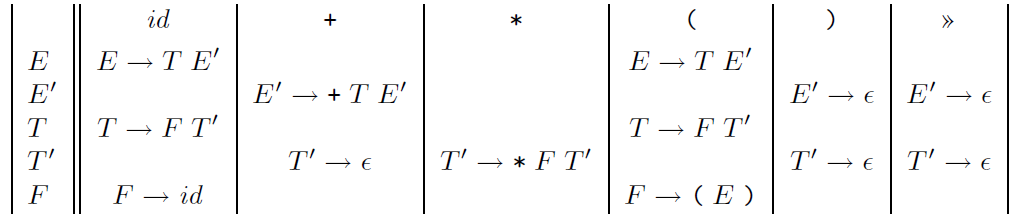
\includegraphics[scale=0.4]{parsing-table.png}

\begin{itemize}
\item For each terminal (see first row), we need a stack pop action.
\item For each non-terminal (see first column), we need one or more expand actions.
\end{itemize}

\end{frame}

\begin{frame}[fragile]{LL(1) parsing - Constructing the parser - Step 2}

\begin{itemize}
\item We'll need a class for each terminal:

\end{itemize}

\begin{lstlisting}[mathescape=true, escapechar=!]
class Id    old new|old$\rightarrow$new where id::String$\rightarrow$old$\rightarrow$ CPS new
class Add   old new|old$\rightarrow$new where !\texttt{+}!::old$\rightarrow$ CPS new
class Mul   old new|old$\rightarrow$new where !\texttt{*}!::old$\rightarrow$ CPS new
class Open  old new|old$\rightarrow$new where !\texttt{(}!::old$\rightarrow$ CPS new
class Close old new|old$\rightarrow$new where !\texttt{)}!::old$\rightarrow$ CPS new
class Endquote old where $\gg$::old$\rightarrow$ Expr
\end{lstlisting}

\end{frame}

\begin{frame}[fragile]{LL(1) parsing - Constructing the parser - Step 2}

\begin{itemize}
\item Instances for pop actions:
\end{itemize}

\begin{lstlisting}[mathescape=true, escapechar=!]
instance Id (I $\alpha$) $\alpha$ where
  id s (I ctx) = return (ctx (Id s))
instance Add (A $\alpha$) $\alpha$ where
  !\texttt{+}! (A ctx) = return ctx
instance Mul (M $\alpha$) $\alpha$ where
  !\texttt{*}! (M ctx) = return ctx
instance Open (O $\alpha$) $\alpha$ where
  !\texttt{(}! (O ctx) = return ctx
instance Close (C $\alpha$) $\alpha$ where
  !\texttt{)}! (C ctx) = return ctx
instance Endquote Expr where
  $\gg$ e = e
\end{lstlisting}

\end{frame}

\begin{frame}[fragile]{LL(1) parsing - Constructing the parser - Step 2}

\begin{itemize}
\item Instances for expand actions, taking Id as an example:
\end{itemize}

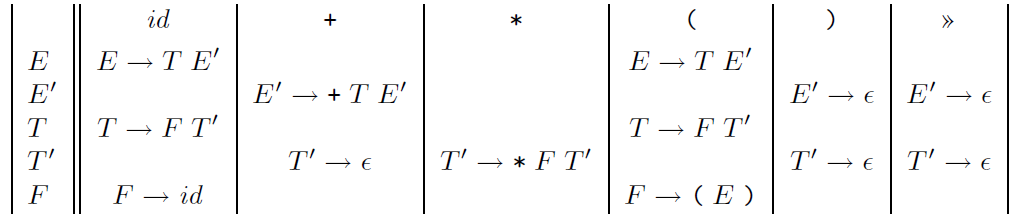
\includegraphics[scale=0.4]{parsing-table.png}
% Each entry of the parsing table gives rise to one instance declaration

\begin{lstlisting}[mathescape=true, escapechar=!]
instance Id (E $\alpha$) (T' (E' $\alpha$)) where
  id s (E ctx) = id s (T ($\lambda$t$\rightarrow$E'($\lambda$e'$\rightarrow$ctx(e' t))))
instance Id (T $\alpha$) (T' $\alpha$) where
  id s (T ctx) = id s (F ($\lambda$f$\rightarrow$T'($\lambda$t'$\rightarrow$ctx(t' f))))
instance Id (F $\alpha$) $\alpha$ where
  id s (F ctx) = id s (I ($\lambda$v$\rightarrow$ctx v))
\end{lstlisting}

\begin{itemize}
\item Expansion phase is E $\rightarrow$ T E' $\rightarrow$ F T' E' $\rightarrow$ id T' E'.
\item The instance head always reflects the parsing state after the final pop action (in this case, this is the $id$ terminal).
\end{itemize}

\end{frame}

\section{LR(0) parsers}

\subsection{Example grammar}

\begin{frame}[fragile]{LR(0) parsing - Our example grammar}

\begin{itemize}
\item LR(0) parsers are tricky to do by hand, so we'll use a very simple grammar: balanced parentheses.

\begin{lstlisting}[mathescape=true, escapechar=!]
P $\rightarrow \epsilon$|!\texttt{(}!P!\texttt{)}!
\end{lstlisting}

\item Abstract syntax is our Tree datatype: P $\rightarrow \epsilon$ is a Leaf, P $\rightarrow$ P\texttt{(}P\texttt{)} is a Fork.

\item The above grammar converts to the following LR(0) automaton:

\end{itemize}

\begin{center}
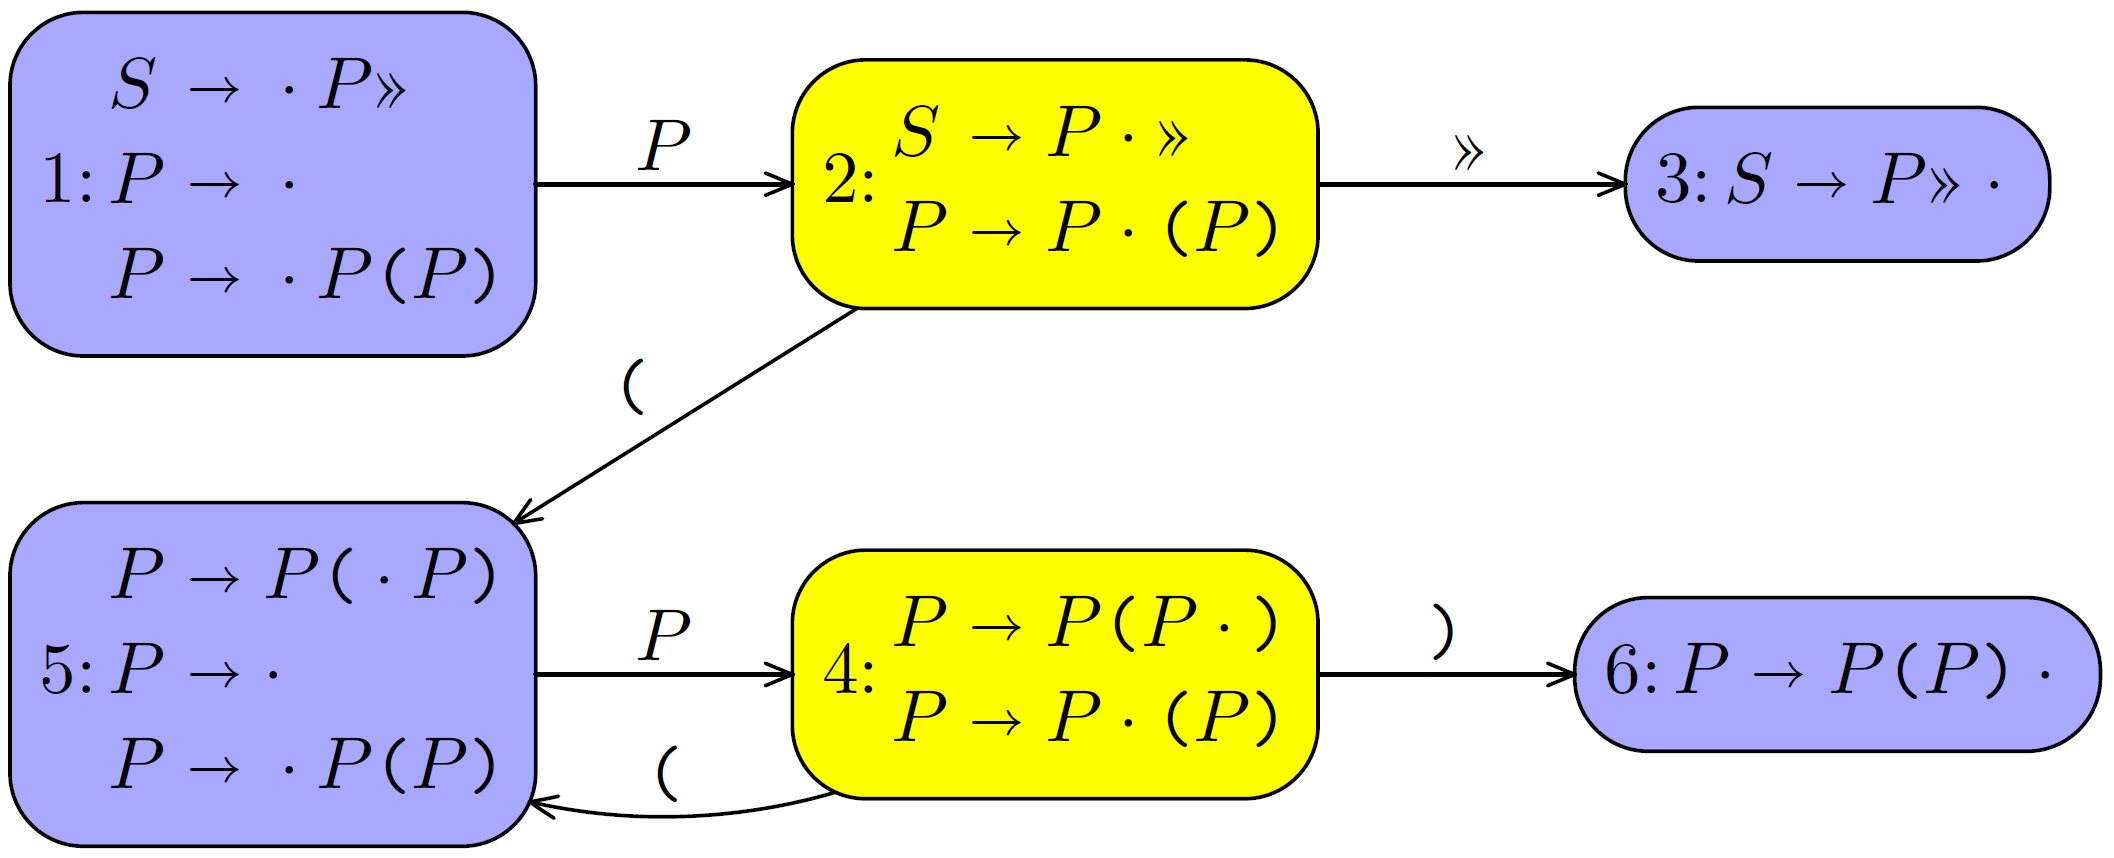
\includegraphics[scale=0.18]{lr0-automaton.png}
\end{center}

\end{frame}

\subsection{LR(0) Automatons 101}

\begin{frame}[fragile]{LR(0) parsing - LR(0) Automatons 101}

\begin{center}
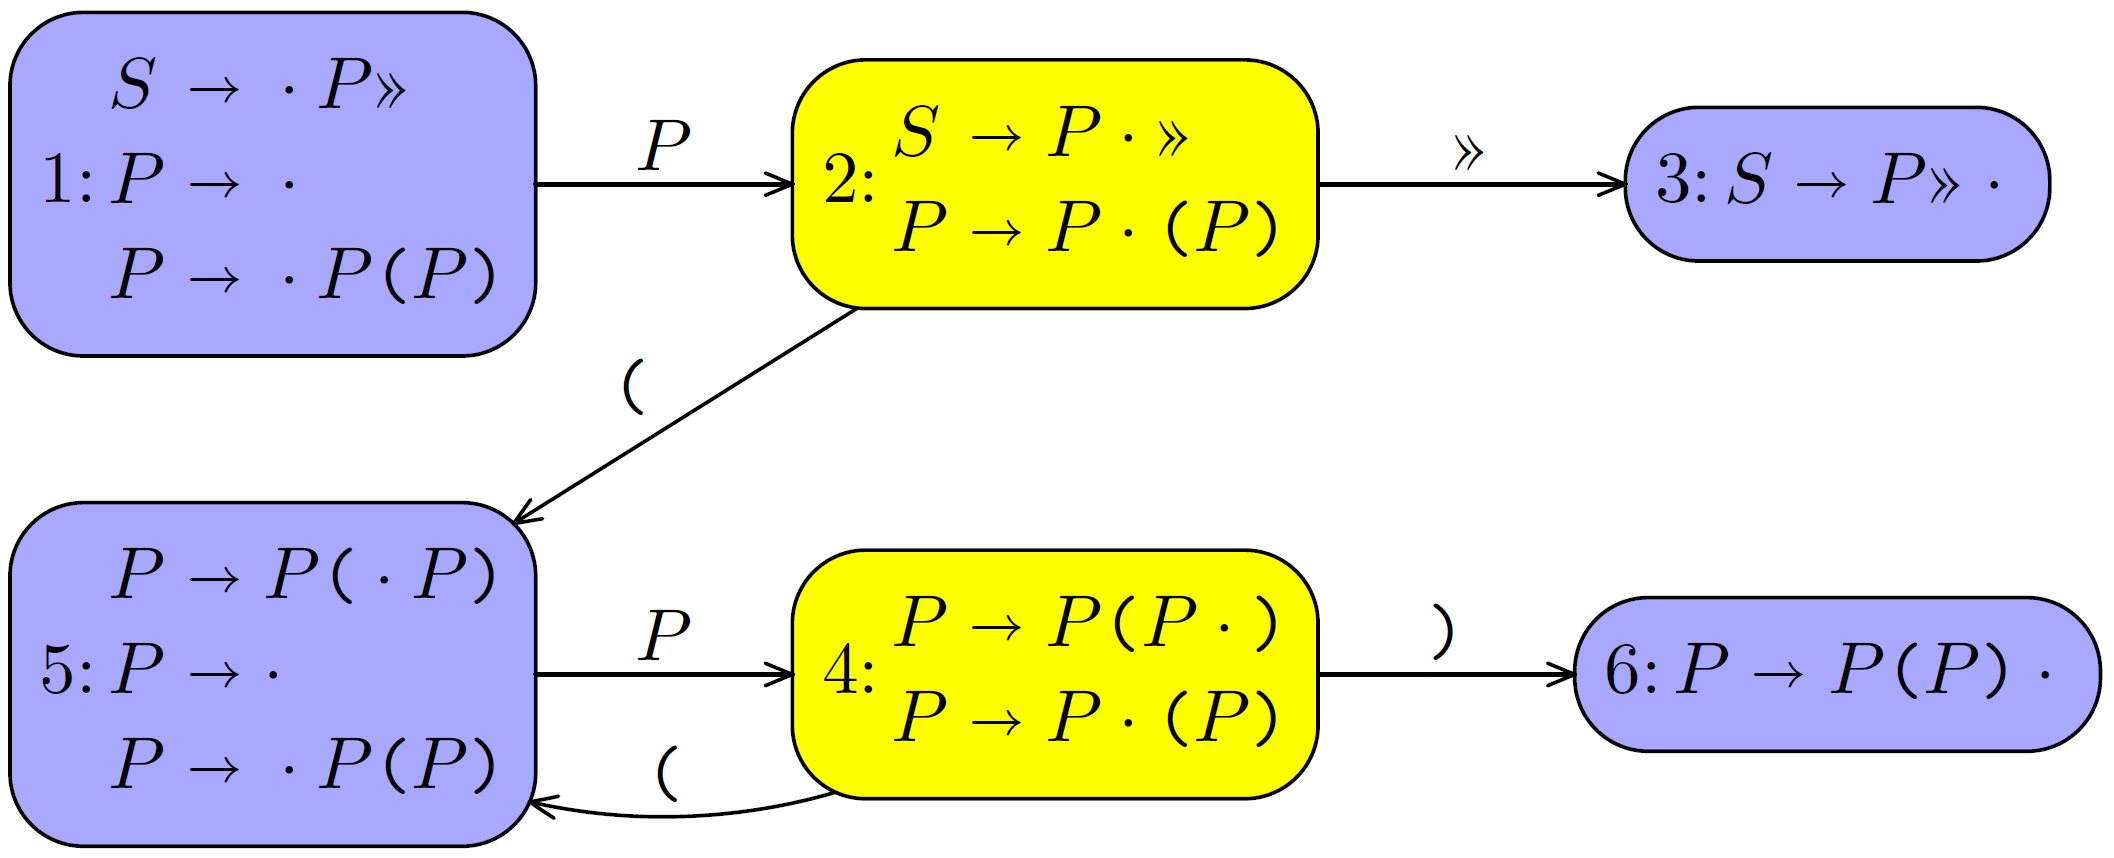
\includegraphics[scale=0.18]{lr0-automaton.png}
\end{center}

\begin{itemize}

 \item An LR parser's stack contains what we've already seen (like postfix).

\item Dots delineate what we've seen and expect to see.
\begin{itemize}
\item Dot before a terminal: \textbf{shift} state, in yellow. Parser consumes the token and pushes it onto the stack.
\item Dot before a non-terminal: \textbf{reduce} state, in blue. RHS of a production is on the stack, we replace it with the LHS.
\end{itemize}

\end{itemize}

\end{frame}

\begin{frame}[fragile]{LR(0) parsing - LR(0) Automatons 101}

\begin{center}
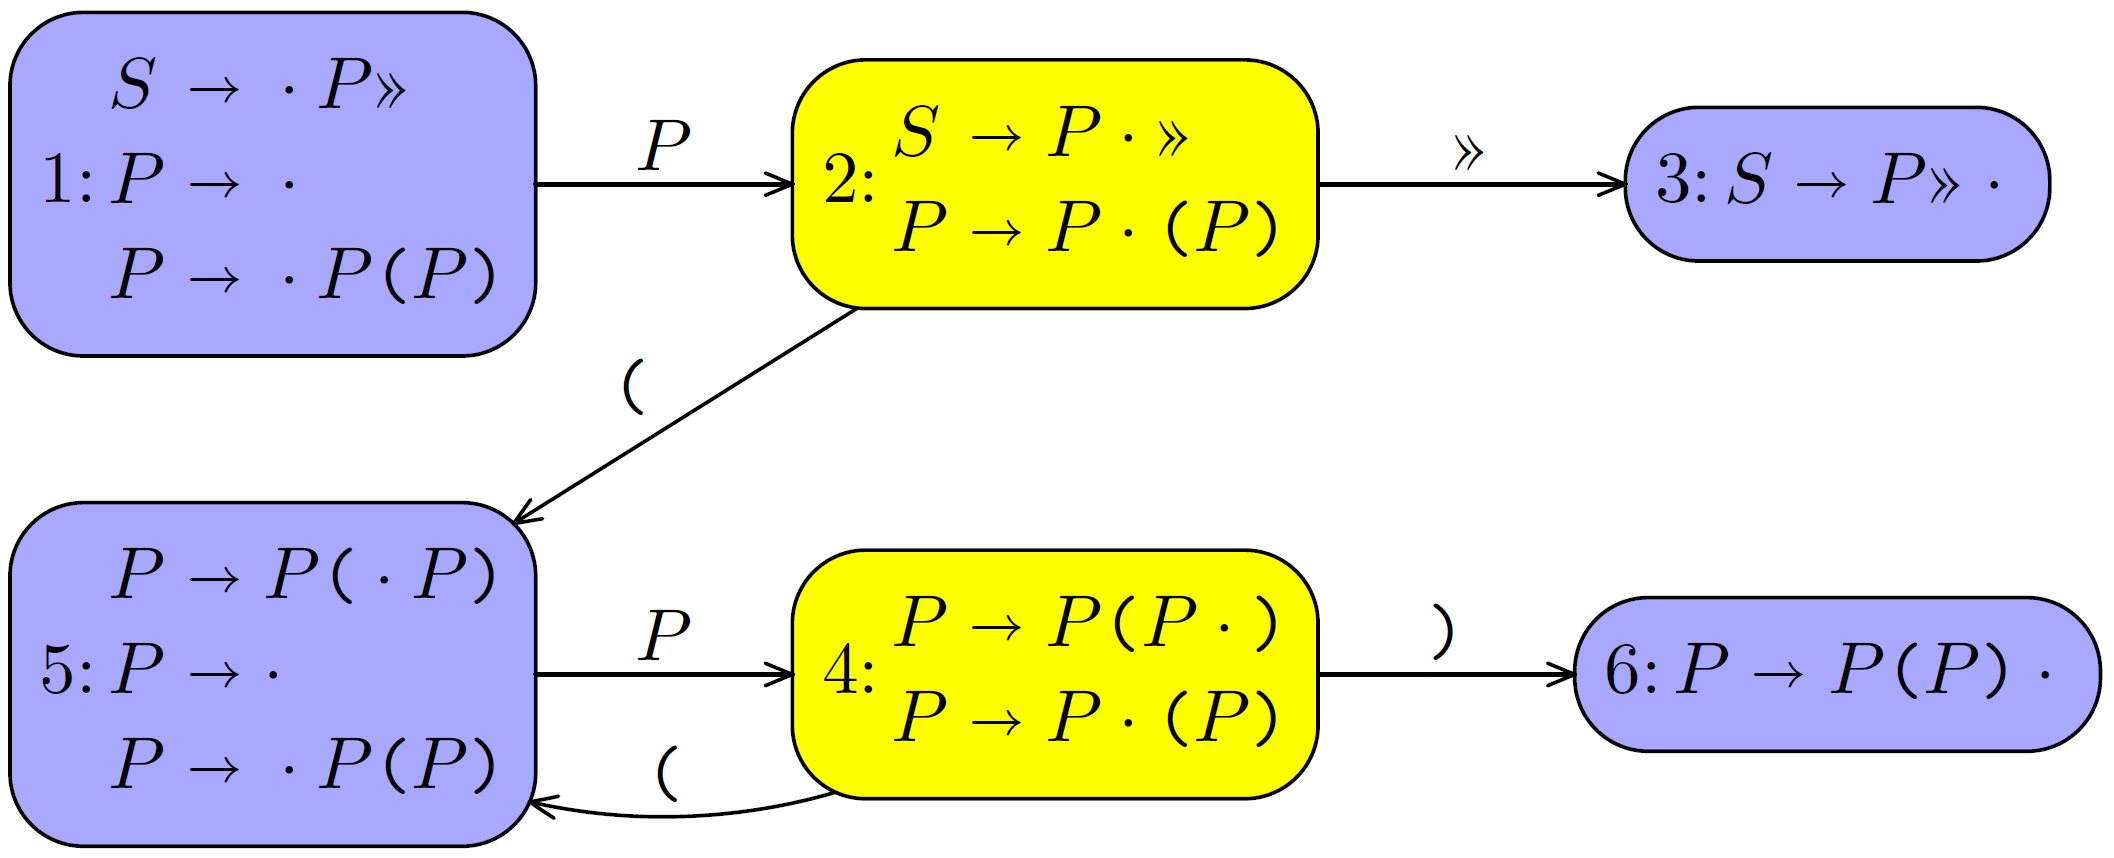
\includegraphics[scale=0.18]{lr0-automaton.png}
\end{center}

\begin{itemize}

\item In our example, the first step is to reduce P $\rightarrow \epsilon$, moving from state 1 to state 2.
\item In state 2, we can shift either '$\gg$' or '\texttt{(}'.
\item Each transition is recorded on the stack. We need this information during reductions.

\end{itemize}

\end{frame}

\begin{frame}[fragile]{LR(0) parsing - LR(0) Automatons 101}

\begin{center}
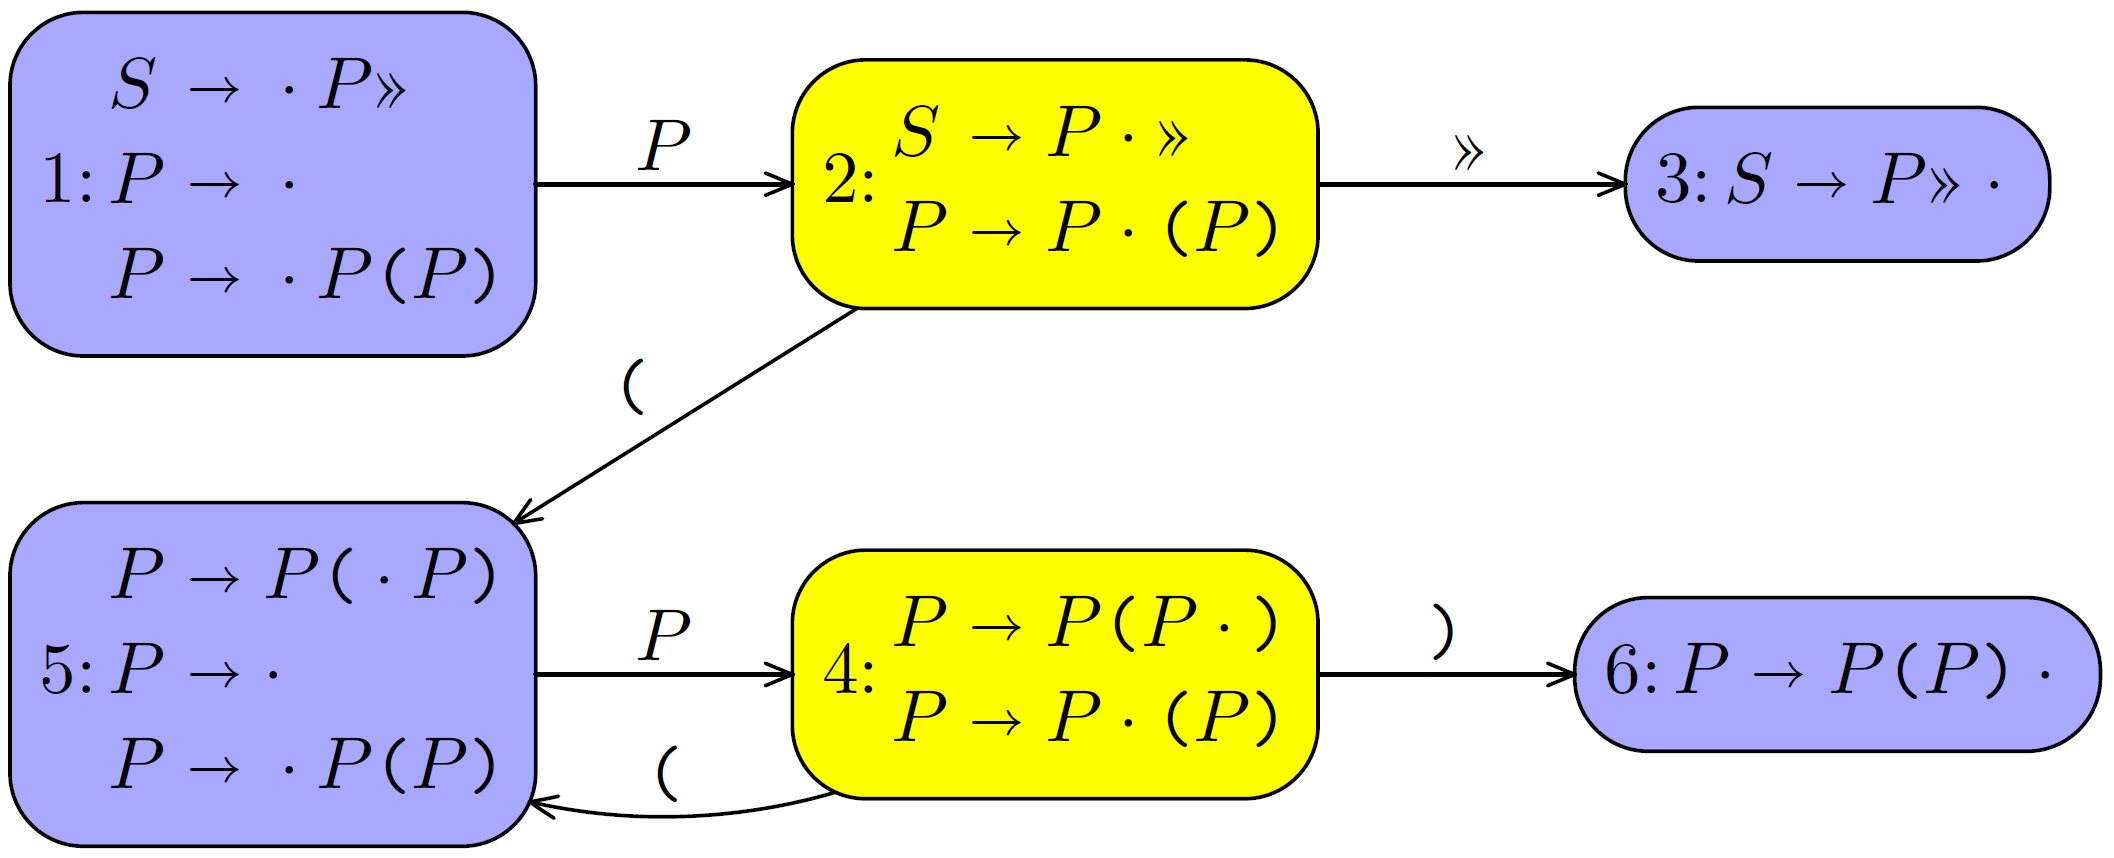
\includegraphics[scale=0.18]{lr0-automaton.png}
\end{center}

\begin{itemize}

\item Consider state 6: there are two sequences of moves that end in this state:
\begin{itemize}
\item $1 \xrightarrow{P}2 \xrightarrow{(}5 \xrightarrow{P}4 \xrightarrow{)}6$
\item $5 \xrightarrow{P}4 \xrightarrow{(}5 \xrightarrow{P}4 \xrightarrow{)}6$
\end{itemize}

\item We need to remove RHS (P $\rightarrow$ P\texttt{(}P\texttt{)}) from the stack. We can end up in 1 or 5. Then, we need to add LHS (P). We can end up in 2 or 4. In general, there are several transitions for a single production.

\end{itemize}

\end{frame}

\subsection{Constructing the parser}

\begin{frame}[fragile]{LR(0) parsing - Constructing the parser - Data types}

\begin{itemize}

\item Parser state = stack of LR(0) states.
\item Each state carries the semantic value of the symbol that annotates the incoming edge(s) of that state.

\begin{lstlisting}[mathescape=true, escapechar=!]
data $S_1$ = $S_1$ !\textcolor{olivegreen}{- - S}!
data $S_2$ st = $S_2$ Tree st !\textcolor{olivegreen}{- - P}!
data $S_3$ st = $S_3$ st !\textcolor{olivegreen}{- - $\gg$}!
data $S_4$ st = $S_4$ Tree st !\textcolor{olivegreen}{- - P}!
data $S_5$ st = $S_5$ st !\textcolor{olivegreen}{- - \texttt{(}}!
data $S_6$ st = $S_6$ st !\textcolor{olivegreen}{- - \texttt{)}}!
\end{lstlisting}

\end{itemize}

\end{frame}

\begin{frame}[fragile]{LR(0) parsing - Constructing the parser - State transitions}

\begin{itemize}

\item Each state is translated into a function:
\begin{itemize}
\item Shift states delegate control to the next active terminal.
\item Reduce states pop the RHS transitions and push the LHS transitions. If there are several possible transitions, we use a type class.
\end{itemize}

\end{itemize}

\begin{lstlisting}[mathescape=true, escapechar=!,basicstyle=\small]
quote = $state_1$ $S_1$ !\textcolor{olivegreen}{- - start}!
$state_1$ st = $state_2$ ($S_2$ Leaf st) !\textcolor{olivegreen}{- - reduce}!
$state_2$ = return st !\textcolor{olivegreen}{- - shift}!
$state_3$ ($S_3$($S_2$ t $S_1$)) = t !\textcolor{olivegreen}{- - accept}!
$state_4$ st = return st !\textcolor{olivegreen}{- - shift}!
$state_5$ st = $state_4$ ($S_4$ Leaf st) !\textcolor{olivegreen}{- - reduce}!
class $State_6$ old new | old $\rightarrow$ new where
  $state_6$ :: old $\rightarrow$CPS new !\textcolor{olivegreen}{- - reduce}!
instance $State_6$ ($S_6$($S_4$($S_5$($S_2$ $S_1$)))) ($S_2$ $S_1$) where
  $state_6$ ($S_6$($S_4$ u($S_5$ ($S_2$ t $S_1$))) = $state_2$ ($S_2$ (Fork t u) $S_1$)
instance $State_6$ ($S_6$($S_4$($S_5$ ($S_4$($S_5$ st))))) ($S_4$($S_5$ st)) where
  $state_6$ ($S_6$($S_4$ u($S_5$ ($S_4$ t ($S_5$ st))))) = $state_4$ ($S_4$ (Fork t u) ($S_5$ st))
\end{lstlisting}

\end{frame}

\begin{frame}[fragile]{LR(0) parsing - Constructing the parser - State transitions}

\begin{itemize}

\item If a terminal annotates more than one edge, we also need a type family:
\end{itemize}

\begin{lstlisting}[mathescape=true, escapechar=!]
class Open old new | old $\rightarrow$ new where
  !\texttt{(}! :: old $\rightarrow$ CPS new
instance Open ($S_2$ st) ($S_4$($S_5$($S_2$ st))) where
  !\texttt{(}! st@($S_2$ _ _) = $state_5$ ($S_5$ st)
instance Open ($S_4$ st) ($S_4$($S_5$($S_4$ st))) where
  !\texttt{(}!  st@($S_4$ _ _) = $state_5$ ($S_5$ st)
!\texttt{(}! st@($S_4$ _ _) = $state_6$ ($S_6$ st)
endquote st@($S_2$ _ _) = $state_3$ ($S_3$ st)
\end{lstlisting}

\begin{itemize}
\item Instance types reflect the stack modifications up to the next shift state.
\item For example, '\texttt{(}' moves from $S_2$ to $S_5$ and then to $S_4$.
\end{itemize}

\end{frame}

\begin{frame}[fragile]{Conclusion}

\begin{itemize}
\item With quotations, terminal symbols turn active and become the driving force of the parsing process.
\item We can construct different kinds of (anti-)quotation parsers in Haskell using the CPS monad.
\item Different state types correspond to different kinds of parsers.
\item Using type-level representations of symbols, we can provide statically-checked type safety.
\item Caveat: Syntax errors become type errors, which may be hard to decipher.
\end{itemize}

\end{frame}

\begin{frame}[fragile]{Thanks for listening!}

\begin{center}
\large Questions?
\end{center}

\end{frame}

\end{document}